\chapter{Background \& Literature Overview}
\label{lit review}

The typical multicellular organism stores its genetic code as deoxyribonucleic acid (DNA), found identically in all its somatic cells (unless \textit{de novo} mutations occur). DNA is a biological polymer, consisting of a double-stranded polynucleotide chain. Each nucleotide monomer consists of a phosphate group, deoxyribose (a five-carbon sugar), and one of four nucleobases: adenine (A), cytosine (C), guanine (G), or thymine (T). These two strands are held together with a series of hydrogen bonds between the nucleobases, forming Watson-Crick base pairs. %On opposite strands, adenine and thymine form double hydrogen bonds, while guanine and cytosine form a stronger triple hydrogen bond.

DNA is just the general starting point in a series of information transfers described by the \textit{Central Dogma of Molecular Biology}, which the cell uses to ultimately produce its molecular products \citep{cobb201760}. Through the process of \textit{transcription}, the code from one strand of DNA is transferred onto a primary ribonucleic acid (RNA) transcript. RNA is similar to DNA except that it is single-stranded, has ribose as its five-carbon sugar and uses the nucleobase \textit{uracil} instead of \textit{thymine}. This primary transcript is modified into ribosomal RNA (rRNA), transfer RNA (tRNA) or messenger RNA (mRNA). All three are involved in \textit{protein synthesis}, although mRNA is especially relevant to this dissertation since the protein sequence can be deduced from the mRNA sequence. These molecular products shape the cell's appearance, define how it interacts with external or internal stimuli, and allows it to perform its intended functions. They give each cell type a characteristic RNA profile which can be measured through RNA-seq (Described in Section ???).

% the intro for this is pretty good: https://www.nature.com/articles/s41368-021-00146-0#:~:text=Bulk%20RNAseq%20studies%20average%20global,next%20generation%20of%20RNA%20sequencing.

\section{Differentiation Pathways in the Haematopoietic System}
. Acute leukaemia occurs earlier in the differentiation pathway, allowing the blasts to divide more rapidly. \autoref{fig:cell_differentiation} shows the mature cell types that result from myeloid and lymphoid cell lineages, which both share \ac{HSC} as the common progenitor cell type.

\begin{figure}[!ht]
    \centering
    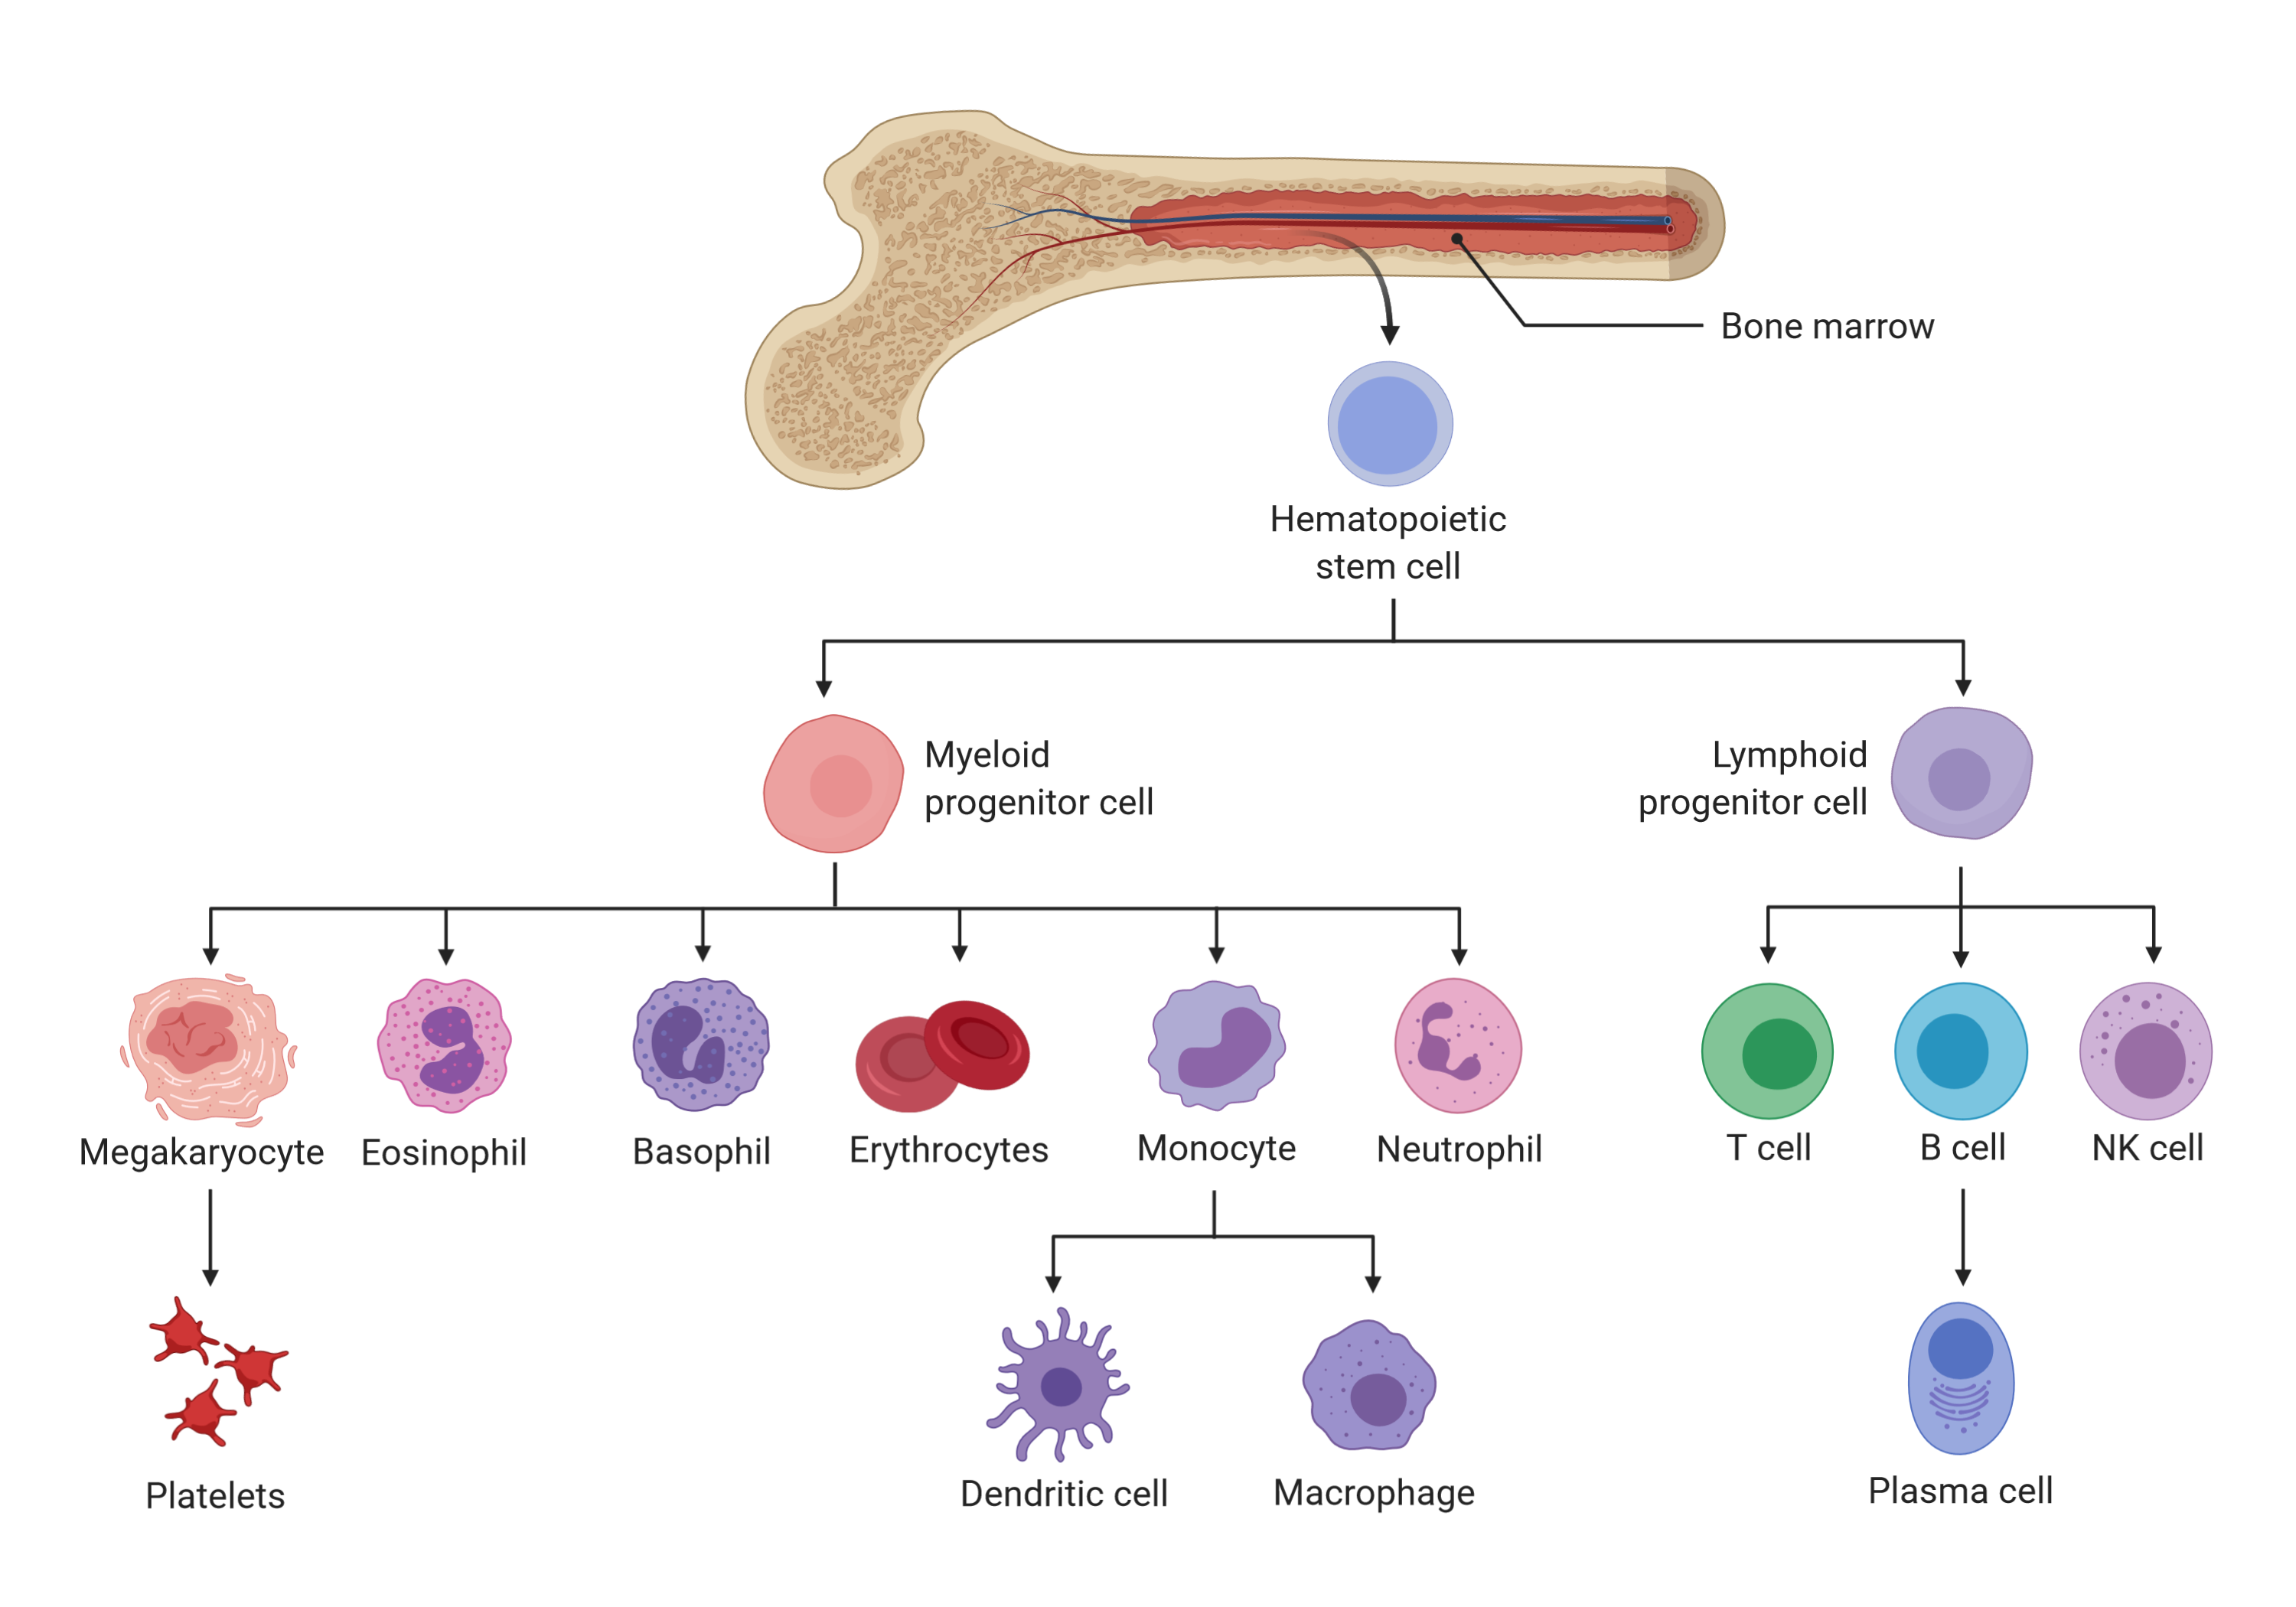
\includegraphics[width=1\textwidth]{cell_differentiation}
    \caption[Stem cell differentiation]{An overview of the main branches of haematopoietic stem cell differentiation pathways showing the myeloid and lymphoid lineages. Created using \href{https://biorender.com/}{BioRender.com}. } 
    \label{fig:cell_differentiation}
\end{figure}


\section{Acute Myeloid Leukaemia}

\ac{AML} is an aggressive form of cancer which is characterised by its rapid proliferation of myeloblasts. This occurs when undifferentiated myeloid cells acquire mutations which hinder further differentiation but allows for their clonal proliferation \citep{Khwaja2016}. This comes at the expense of the production of their healthy, differentiated counterparts: erythrocytes, platelets and granulocytes \citep{Khwaja2016}. It is an exception to cancers in that it does not form a tumour, which is usually analysed to determine the severity. Instead \ac{AML} is staged according to its subtype and other variables \citep{ACS2018}. It is the most common form of acute leukaemia, with an incidence rate of 4.3 per 100,000 in the United States \citep{Kouchkovsky2016}. One of the main risk factors is age, with a median age of diagnosis of 70 years, and with a slight male predominance \citep{juliusson2009age, Khwaja2016}. Acute myeloid leukaemia is synonymous with acute myelogenous leukemia, acute myelocytic leukemia, or acute nonlymphocytic leukemia.

%Summary of leukaemia: https://www.cancer.net/cancer-types/leukemia-acute-myeloid-aml/introduction

\subsection{Classification and Subtypes}
\label{Classification and Subtypes}
\ac{AML} is one of four main branches of leukaemia classification, the others being Acute Lymphoblastic Leukaemia (ALL), Chronic Myeloid Leukaemia (CML) and Chronic Lymphoblastic Leukaemia (CLL) \citep{leukaemiabook}. Despite their cytogenic differences, there have been multiple reports of chronic leukaemia types transitioning into the more aggressive, acute form over time \citep{kaur2016rapid, frenkel1981acute, jacobs1984acute}. Treatment may vary depending on the subtype of the disease, which is why a rigid classification system and correct identification is important \citep{leukaemiabook}.

Each of these four leukaemia subtypes is subdivided into more specific classifications. \ac{AML} in particular is genetically and morphologically heterogeneous and can involve any single or a combination of myeloid lineages \citep{whoclassification, Kouchkovsky2016}. 

\subsubsection{The FAB classification system}
The \ac{FAB} classification, first produced in 1976, was an early attempt to distinguish subtypes of \ac{AML} \citep{bennett1976proposals}. The divisions were based on cell morphology and the relative quantities of myeloblasts and erythroblasts \citep{acsamlsubtypes}.

%Maybe lookup cool table latex tutorials to make it nicer (colours maybe?)
\begin{table}[h]
\centering
\caption{The FAB classification of AML.}
\label{tab:FABclassification}
\begin{tabular}{lll}
\hline
M0 & Undifferentiated acute myeloblastic leukemia        &  \\ 
M1 & Acute myeloblastic leukemia with minimal maturation &  \\
M2 & Acute myeloblastic leukemia with maturation         &  \\
M3 & Acute promyelocytic leukemia (APL)                  &  \\
M4 & Acute myelomonocytic leukemia                       &  \\
M5 & Acute monocytic leukemia                            &  \\
M6 & Acute erythroid leukemia                            &  \\
M7 & Acute megakaryoblastic leukemia                     &  \\ \hline
\end{tabular}
\end{table}

% AML categories are extremely heterogeneous, probably due to high genetic diversity

\subsubsection{The WHO classification system}

A more modern, and now more widely used system, is that devised in the \textit{\ac{WHO} Classification of Tumors of Hematopoietic and Lymphoid Tissues}, now in its revised 4th edition \citep{whoclassification}. \ac{AML} is here defined as having >20\% of the cells in the bone marrow being myeloblasts. The \ac{WHO} based their classification on a mixture of genetic, morphological and cytochemical criteria and based on the presence of other conditions. They define seven subcategories:

\begin{enumerate}
\item AML with recurrent genetic abnormalities
\item AML with myelodysplasia-related changes (MRC)
\item Therapy-related myeloid neoplasms (t-MN)
\item AML related to previous chemotherapy or radiation
\item Myeloid sarcoma (also known as granulocytic sarcoma or chloroma)
\item Myeloid proliferations related to down syndrome (DS)
\item AML with chromosomal translocations and inversions
\end{enumerate}

These may be further classified according to their specific genetic or karyotypic abnormalities \citep{whoclassification}. Cases which do not fall into any of the above groups, are labelled as 'AML, not otherwise specified (NOS)' and are subject to a form of classification similar to the \ac{FAB} \citep{ACS2018}. Cases classified as having 'recurrent genetic abnormalities' are often sub-categorised and described according their their abnormality (similar to table \ref{tab:karyotype}, although not all are officially recognised as 'recurring abnormalities').

%https://emedicine.medscape.com/article/2006750-overview?reg=1
%https://www.ncbi.nlm.nih.gov/books/NBK560490/

\subsection{Pathogenesis}
The genetic abnormalities leading to \ac{AML} are heterogeneous and complex, meaning that there are many different combinations of causative genetic or cytogenetic abnormalities which may lead to the \ac{AML} phenotype \citep{lindsley2015acute, whoclassification}. The genetic and karyotypic profile can have profound prognostic impact, affecting both therapeutic strategy and survival rate \citep{mrozek2000prognostic, whoclassification}. 

\subsubsection{Cytogenic Abnormalities}
Approximately 55\% of \ac{AML} patients have at least one cytogenic abnormality \citep{meyer2014translational}.  \cite{stolzel2016karyotype} note that patients with 3 unrelated cytogenic abnormalities, have a worse overall survival rate than \ac{AML} patients with a normal karyotype, and that the patients at most risk had $ \geq $4 unrelated cytogenic abnormalities. There are some exceptions, where the presence of certain abnormalities actually \textit{increases} survival rate with good response to treatment (Table \ref{tab:karyotype}). 

\begin{landscape}
	\pagestyle{empty} % to remove headers on the side	
\begin{table}[h]
\label{tab:karyotype}
    \centering
    \caption{Recurrent abnormalities in AML and their effects. This table makes use of the International System for Human Cytogenomic Nomenclature (ISCN) to describe chromosomal abnormalities \citep{ISCN}. The information given prior to the parentheses denotes the type of chromosomal abnormality (for example \textit{t} for translocation, and \textit{inv} for inversion). The contents of the first pair of parenthesis refer to the affected chromosome(s). The second pair of parentheses, if present, refers to the specific part of the respective chromosome(s) affected (the short arm \textit{p} or the long arm \textit{q}, and which region or band of these arms).}
    \begin{tabular}{lllllllllllll}
    \toprule
        \textbf{Aberration} & \textbf{Prognosis} & \textbf{Fusion Genes} & \textbf{Note} & \textbf{Reference}  & ~ \\ \midrule
        t(8;21)(q22;q22) & Favourable & RUNX1, RUNX1T1 & Common (\textasciitilde 5\% of all AML) & \cite{reikvam2011acute}  & ~ \\ 
        ~ & ~ & ~ & ~ & \cite{peterson20048}  & ~ \\ \hline
        inv(16)(p13;q22) & Favourable & CBFB, MHY11 & Common & \cite{plantier1994inv}  & ~ \\ 
        t(16;16)(p13;q22) & ~ & ~ & ~ & \cite{shigesada2004mechanism}  & ~ \\ \hline
        t(15;17)(q24;q21) & Favourable & PML, RARA  & Common (\textasciitilde 10\% of adult AML) & \cite{de2014rara}  & ~ \\ 
        ~ & ~ & ~ & ~ &   & ~ \\ \hline
        t(9;11)(p22;q23) & Poor & KMT2A, MLLT3 & Frequency decreases with age & \cite{chandra2010acute}  & ~ \\ 
        ~ & ~ & ~ & ~ & \cite{metzler2004emergence}  & ~ \\ \hline
        t(6;9)(p23;q34) & Poor & DEK, CAN/NUP214 & Rare, associated with an internal tandem & \cite{chi2008acute}  & ~ \\ 
        ~ & ~ & ~ &  duplication (ITD) mutation on FLT3 &   & ~ \\ \hline
        inv(3)(q21.3;q26.2) & Poor & RPN1, MECOM & Rare, low response to standard  & \cite{sitges2020acute} & ~ \\ 
        t(3;3)(q21.3;q26.2) & ~ & ~ & chemotherapy & ~ & ~ \\ \hline
        t(1;22) (p13;q13) & Poor & RBM15, MKL1 & Rare, almost exclusively found in infants   & \cite{carroll1991t} & ~ \\ 
        ~ & ~ & ~ &  with acute megakaryocytic leukaemia & \cite{bernstein2000nineteen} & ~ \\ \hline
        Monosomy  & Very poor & / & Loss of chromosome, frequency increases & \cite{breems2008monosomal} & ~ \\ 
        ~ & ~ & ~ &  with age &   & ~ \\ \bottomrule
    \end{tabular}
\end{table}
\end{landscape}


%t(8;21) is a frequently oc­curring aberration in acute AML. It involves the fusion of the RUNX1 (runt-related transcription factor 1) gene on chromosome 21q22 and the RUNX1T1 (runt-related transcription factor 1; translocated to 1) gene on chromosome 8q22, resulting in the formation of the hybrid gene RUNX1/RUNX1T1. AML with t(8;21)(q22;q22), RUNX1/RUNX1T1 generally shows maturation in the myeloid lineage and is found in approximately 5\% of cases of AML. cite:https://atlasgeneticsoncology.org/haematological/1019/t(8;21)(q22;q22)-runx1-runx1t1

% SUMMARY OF CHROMOSOMAL TRANSLOCATIONS AND THEIR OUTCOMES: https://www.cancer.org/cancer/acute-myeloid-leukemia/detection-diagnosis-staging/how-classified.html


\subsubsection{Genetic Abnormalities}

If we reduce our frame of reference to the genetic level, we find that the aforementioned structural variants (Table \ref{tab:karyotype}) can trigger the activation of an \textit{oncogene}, or their fusion products (Table \ref{tab:karyotype}) can become an oncogene themselves. Some genes have the potential to cause cancer under abnormal conditions and are called \textit{proto-oncogenes}, and if said conditions are met, become the carcinogenic oncogenes. This carcinogenicity can be triggered by either a structural variant, a \ac{SNP} or gene amplification \citep{tabin1982mechanism}. This can cause up-regulation, over-activity or a change in function of the respective protein \citep{tabin1982mechanism}. These proteins are often the targets of cancer drugs \citep{liu2004new}.

Cells have evolved mechanisms to prevent carcinogenesis, through \textit{tumour suppressor genes}. These genes are typically involved in the regulation of cell division, DNA repair or induction of apoptosis. While proto-oncogenes require their up-regulation to induce cancer, tumour suppressor genes require down-regulation or complete deactivation. \cite{knudson1971mutation} suggested a 'two-hit hypothesis', that most tumour suppressor genes require the deactivation of both alleles for carcinogenesis to occur. Knudson theorised that early onset retinoblastoma (cancer of the retina) was caused by an inherited mutation (the first 'hit') and a second acquired mutation (the second 'hit'). Knudson explained late-onset of the disease as being non-inherited, with both 'hits' being acquired. 

%The TP53 gene is the most frequently mutated gene (>50%) in human cancer, indicating that the TP53 gene plays a crucial role in preventing cancer formation.[6] https://doi.org/10.2147%2FOTT.S53876
\clearpage
\begin{table}[H]
\label{tab:genetic abnormalities}
    \centering
    \caption{Recurring genetic abnormalities in \ac{AML}. Compiled and adapted from \cite{dinardo2016mutations} Table 1 and \cite{lindsley2015acute} Figure 2.}
    \begin{tabular}{llllllllll}
    \toprule
\textbf{Role} & \textbf{Role description} & \textbf{Mutated genes} &  &  \\ \midrule
Signalling pathways & Internal or external & NRAS, KRAS, PTPN11, &  &  \\
 & chemical communication & NF1, CBL, KIT, FLT3 &  &  \\ \hline
DNA methylation & Epigenetic modifier, adds & DNMT3A, TET2, IDH1, &  &  \\
 & methyl groups to DNA & IDH2 &  &  \\ \hline
Chromatin modifiers & Epigenetic modifier, & ASXL1, EZH2, BCOR &  &  \\
 & remodels chromatin &  &  &  \\ \hline
Transcription factors & Involved in transcribing & CEBPA, RUNX1, GATA2 &  &  \\
 & DNA into RNA &  &  &  \\ \hline
Tumour suppressors & DNA repair, initiation of & TP53 &  &  \\
 & apoptosis, halting cell growth &  &  &  \\ \hline
Spliceosome complex & Ribonucleoprotein complex & SRSF2, U2AF1, SF3B1, &  &  \\
 & involved in splicing RNA & ZRSR2 &  &  \\ \hline
Cohesin complex & Protein complex involved in & STAG2, SMC3, SMC1A, &  &  \\
 & chromatid cohesion & RAD21 &  &  \\ \hline
Others & Other proto-oncogenes & WT1, PHF6, TP53, &  &  \\
 &  & NPM1 &  &  \\ \bottomrule
    \end{tabular}
\end{table}

\subsection{Transcriptomic abnormalities}
Pathways


\subsection{ Treatment Methods}
\label{Treatment Methods}
Surgery, chemotherapy, radiotherapy, immunotherapy and hormone therapy are common treatments used to kill cancer cells. While the specifics are partly dependent on the particular \ac{AML} subtype and the patient's condition, some variation of chemotherapy is standard practice. Treatment is typically split into four phases spread over a period of 2-3 years \citep{malard2020acute}:  

\begin{enumerate}
\item \textbf{Induction} - Uses chemotherapeutic drugs with the intention of achieving complete remission (no symptoms or signs of cancer) and restore normal cellular activity. Cytarabine (AraC) is one of the most commonly used chemotherapeutic drugs for \ac{AML}, often used in conjunction with others such as daunorubicin \citep{Robak2009}.
\item \textbf{Consolidation} - Consists of several short sequential courses of chemotherapy every two weeks, usually using stronger doses.
\item \textbf{Intensification} - Also called reinduction therapy, includes drugs similar to those used during the induction phase.
\item \textbf{Long-term maintenance} - Chemotherapy is performed for 2-3 years after complete remission to prevent, or slow down, the growth of any cancer remnants. At times, a bone marrow or stem cell transplant is sometimes necessary to replenish the supply of healthy hematopoietic cells
\end{enumerate}

In recent decades, advances in our knowledge of cancer biology and the development of more efficient high-throughput sequencing techniques, have lead to the identification of novel treatments which specifically target cancer cells, such as differentiation therapy. A key characteristic of cancer cells is remaining in a stem-cell like state, which allows for their rapid proliferation. Differentiation therapy is a relatively modern approach which attempts to induce the process of differentiation, where the malignant cells mature and lose their ability to proliferate, rendering them virtually harmless. The first successful differentiation agent was \ac{ATRA}, also known as tretinoin, used to treat acute promyelocytic leukaemia (APL) \citep{chomienne1990all}. This revolutionary drug managed to achieve a 90\% survival rate in APL patients, without the severe cytotoxic side-effects of traditional non-targeted chemotherapy \citep{kim2015selection}. There have been many attempts to emulate this with other compounds, with mixed results \citep{nowak2009differentiation}.

\subsection{The Model Cell Line: HL-60 }
A 36-year-old Caucasian woman was being treated for \ac{AML} at the MD Anderson Cancer Center in Texas, 1977, when she consented to being part of a study on her disease. Researchers took a blood sample, from which they extracted blasts for their analysis. Three years later, \cite{gallagher1979characterization} would describe for the first time the HL-60 cell line, now one of the most widely used \ac{AML} cell lines. The cells were described as having primarily neutrophilic and promyelocytic morphology, and thus initially placed into the \ac{FAB}-M3 'acute promyelocytic leukemia' category (see Section \ref{Classification and Subtypes}). Subsequent analysis of the cells' karyotype, performed by \cite{dalton1988hl}, revealed that they lacked the t(15;17) translocation characteristic of \ac{FAB}-M3, and were categorised as \ac{FAB}-M2, but development in nomenclature led the cell-line to finally being placed in the 'AML with maturation' category, using the \ac{WHO} system.

Early karyotypic studies had identified the t(5;17) \citep{von1990double} and t(9;14) translocations, together with a complex structural variant between chromosomes 5, 7, and 16 \citep{liang1999spectral}. A more recent study by \cite{jacob} used genome wide chromatin conformation capture (Hi-C) and RNA-seq to study structural variants in HL-60 genetic branches. They have shown the heterogeneity in HL-60 cell lines, but identified novel structural variants thought to be found in the original HL-60 sample: t(5;7)(q31.2;q32.3), t(5;16)(q33.3;q23.2-q23.3), t(7;16)(q32.3;q24.1), t(9;14)(q31.1;q23.2), and t(5;17)(q11.2;p11.2).

As mentioned in Section \ref{Treatment Methods}, \ac{ATRA} has been a success story in \ac{AML} differentiation therapy, and since its discovery, has been extensively used on HL-60 cells. This has led to the evolution of an ATRA-resistant branch of the HL-60 cell line, which was used during the study \citep{Gatt2016} that laid the foundation for this dissertation. \cite{fu2005effects} were successful in reverting this resistance through gene knockdown of MCL-1, which seems to produce the protein responsible for \ac{ATRA} resistance.

%Pathway analysis


%Read Lucienne's papers and their references
%\section{Phenols in Maltese Extra Virgin Olive Oil}

%In vivo


\section{RNA-seq: \textit{in vitro}}
RNA sequencing (RNA-seq) is the application of a \ac{NGS} technique to measure the quantity of RNA sequences in a biological sample, in a given moment \citep{zhong2009}. While this dissertation deals with the data analysis part of RNA-seq, some background on the origins of said data is essential. RNA-seq has gradually been replacing microarrays as the standard technology in molecular biology to analyse \ac{DGE}. Its main advantage is that it allows for the sequencing of the entire transcriptome, while microarrays only allow for predefined regions to be sequenced \citep{rao2019comparison}. 

Sanger sequencing is considered as the first generation in a series of changes in sequencing technology, developed in 1977 and dominated the nucleic acid sequencing industry for over 30 years \citep{behjati2013next}. Next-generation sequencing (or second generation sequencing) revolutionised the industry, its massively parallel capabilities allowing for greatly increased throughput, sequencing millions of fragments at a time instead of Sanger sequencing's just one. At the time of writing, we are currently in the process of transitioning into the third generation of nucleic acid sequencing, which allows for longer reads (>1000 bp as opposed to 35-600 bp). Longer reads translate to greater overlap between the reads, and thus greater certainty during assembly or alignment, particularly when considering regions of low-complexity or structural variants \citep{rhoads2015pacbio}. 

We should make a distinction between two popular types of RNA-seq: the classic bulk RNA-seq, and single-cell RNA-seq (scRNA-seq). Bulk RNA-seq, which this project has made use of, takes the average gene expression of a sample, which may be composed of many cell types, while scRNA-seq investigates the transcriptome of each individual cell. RNA-seq is traditionally used to profile transcriptomes, but it may be used in the identification of expressed SNPs, identification of novel transcripts, the detection of fused genes and alternative splicing \citep{han2015alternative, zhao2014comparison}. 


% great summary of rna sequencing: https://www.sciencedirect.com/science/article/pii/S0090825818312836#bb0080
% also really good https://www.thieme-connect.com/products/ejournals/html/10.1055/s-0039-1688446

%non coding rna: https://www.mdpi.com/1422-0067/17/12/2080


\subsection{RNA extraction}
The first step in any RNA-seq workflow is the extraction of RNA from the biological sample. This is complicated by the chemical instability of RNA due to its hydroxyl groups at the 2' and 3' positions, facilitating RNase activity (RNA-degrading enzymes) \citep{green2019win}. This issue is compounded by the ubiquity and chemical resilience of RNAses, meaning that special care must be taken to avoid contamination of glassware and instruments that interact with the RNA \citep{green2019win}. One method uses liquid nitrogen to deactivate any RNase enzymes and freeze the samples, which are pulverised to extrude the cell contents \citep{wang1994extraction}. 

The data serving as the basis for this dissertation was provided by \cite{Gatt2016}, who followed the RNeasy® Mini kit \citep{RNeasy} which makes use of an extraction technique called \textit{acid guanidinium thiocyanate-phenol-chloroform} (AGPC) extraction \citep{chomczynski1987single}. This is based on \ac{LLE} \citep{mazzola2008liquid}, where under acidic conditions the cell's RNA partitions into the aqueous phase while the DNA, proteins and lipids partition into the organic phase, aided by centrifugation. The organic phase is composed of phenol (which dissolves the protein) and chloroform (which dissolves the lipids). Guanidinium thiocyanate is part of the kit's buffer solution, and acts as a chaotropic agent, meaning it disrupts water's hydrogen bonds. This is added to the organic phase to disrupt the hydrophobic properties of protein (including RNases), aiding in their denaturation. Ethanol is added to precipitate the RNA and any residual DNA. A spin-column is used to bind nucleic acids to a silica membrane, and wash away any proteins, carbohydrates, fatty acids and any traces of salts, aided by centrifugation \citep{matson2009microarray}. The end-result is a purified aqueous nucleic acid solution. 

RNA concentration is commonly checked through quantitation using a spectrophotometer, which measures the ability of the sample to absorb UV light at wavelengths of 260nm and 280nm. A score is assigned to the sample's ability to absorb each of the two wavelengths, and the purity of the sample is often quantified using the ratio between the two scores (A260/280 ratio). A pure RNA sample should yield an A260/280 ratio of ~2.0 \citep{scientific2013t042}.

An additional quality metric commonly checked before sequencing, is the integrity of the RNA. This can be quantified via the \ac{RIN} algorithm, applied to the results of capillary electrophorisis, which separates the RNA fragments based on their length \citep{schroeder2006rin}. In most labs, the electrophoresis and computation of the \ac{RIN} is performed automatically in an electropherogram \citep{chamieh2015quantitative}. A poor \ac{RIN} may indicate RNase contamination during extraction, that could have degraded the RNA.

\subsection{Library Preparation}
'RNA' is a generic term, which includes both coding and non-coding RNA. Ribosomal RNA (rRNA) is a form of non-coding RNA which comprises 80\% to 95\% of the total RNA \citep{o2013ribosomal, kukurba2015rna} and must be removed before sequencing. 

There are two main competing methods available, each with their unique advantages and restraints: poly-A enrichment and rRNA depletion. The 3' end of messenger RNA (mRNA) undergoes polyadenylation prior to transcription, meaning that a long chain of adenine nucleotides called the \textit{poly-A tail} is added. With poly-A enrichment, RNA fragments with a poly-A tail are enriched with oligo (dT) primers, thus selecting for the mRNA \citep{zhao2014comparison}. The alternative approach is an active removal of the rRNA using commercially available kits, such as the Illumina \textit{Ribo-Zero Plus rRNA Depletion Kit}. These kits use oligonucleotides complementary to the rRNA sequences to reduce their abundance \citep{griffith2015informatics, peano2013efficient}. 

The next two steps are fragmentation and conversion to complimentary DNA (cDNA), the order of which may vary. In the Illumina workflow used to generate the data for this dissertation, the RNA strands were first fragmented, and reverse transcribed to their cDNA counterparts \citep{pease2012rapid}. A short, artificially synthesised oligonucleotide called an \textit{adapter} sequence is ligated to each of the cDNA fragments, using the ligase enzyme, together with sequence motifs such as barcode sequences \citep{pease2012rapid} (\autoref{fig:ngs_clonal_amp}).

%This adapter-ligated cDNA library is typically attached to a flow-cell, amplified and sequenced in a high-throughput sequencing platform which typically results in a FASTQ \citep{cock2010sanger} file. % Include more detail here?

%cDNA synthesis and preparation 
%of an adaptor-ligated sequencing library. The library is 
%then sequenced to a read depth of 10–30 million reads 
%per sample on a high-throughput platform (usually 
%Illumina)

\begin{figure}[!ht]
    \centering
    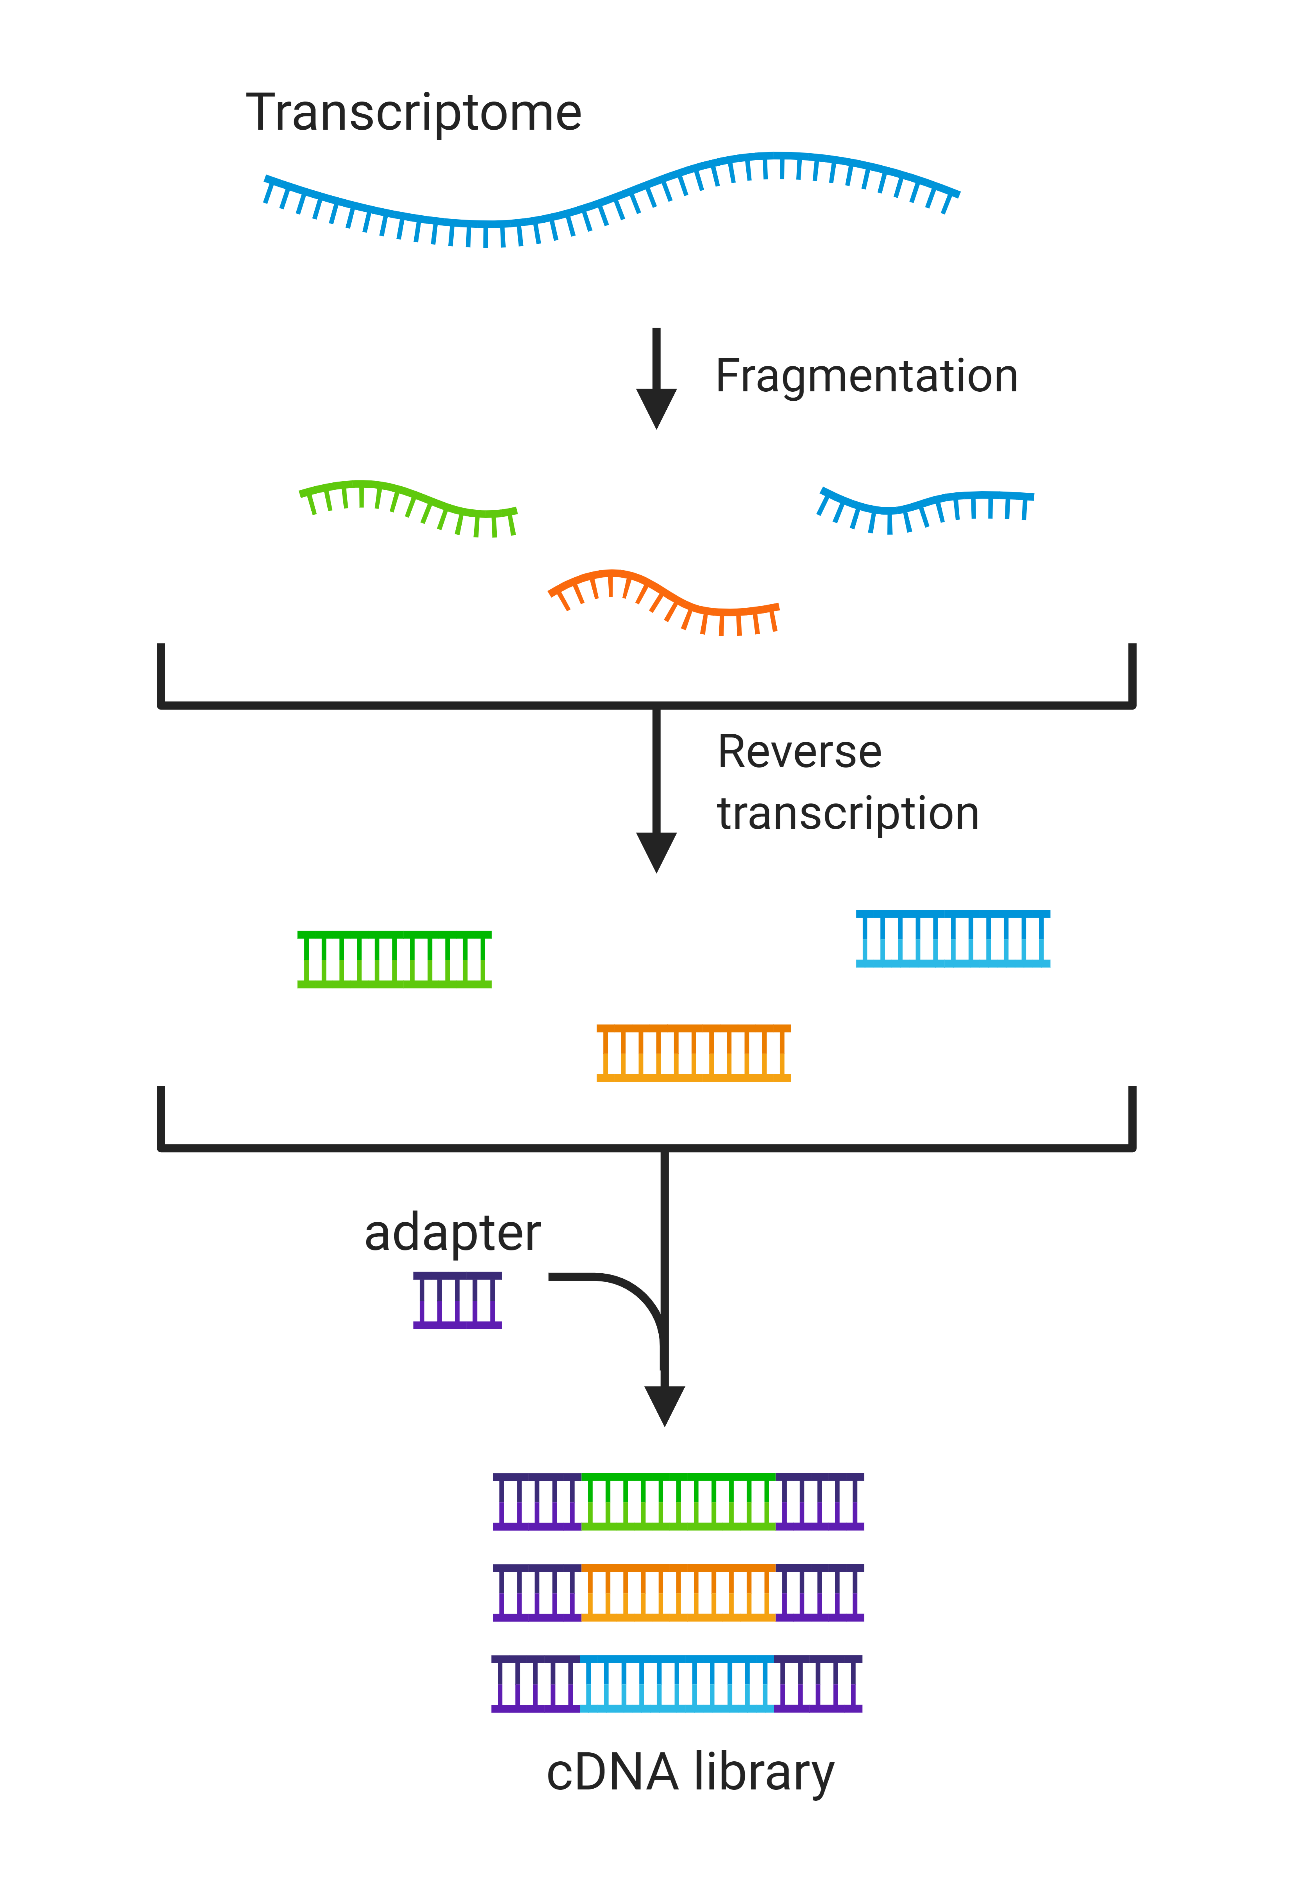
\includegraphics[width=8cm]{ngs_lib_prep}
    \caption[Library preparation]{Illumina library preparation. Created using \href{https://biorender.com/}{BioRender.com}. } 
    \label{fig:ngs_lib_prep}
\end{figure}
\clearpage

\subsection{Clonal amplification}
The following step amplifies the fragments of the cDNA library to a level detectable by the sequencing machine, using a form of \ac{PCR}. The Illumina Sequencing by Synthesis technology makes use of the flow-cell-based method of \textit{bridge amplification} \citep{illumina2010}, as opposed to emulsion PCR, a similar technology used in Ion Torrent Semiconductor Sequencing which makes use of bead surfaces \citep{williams2006amplification}.

In bridge amplification \citep{illumina2010}, the previously prepared adapter-ligated cDNA library is attached to a flow cell, which is a hollow glass slide with multiple channels, coated with a lawn of oligonucleotides (called oligos in short) complimentary to the sequences which form part of the adapters. Strands of cDNA bind to these oligos, and polymerase creates the complement of the hybridised strand. Each double-stranded cDNA molecule is then denatured and enters a number of bridge-amplification cycles. Each molecule is amplified, forming clusters of identical cDNA sequences adjacent to each other (\autoref{fig:ngs_clonal_amp}).

\begin{figure}[!ht]
    \centering
    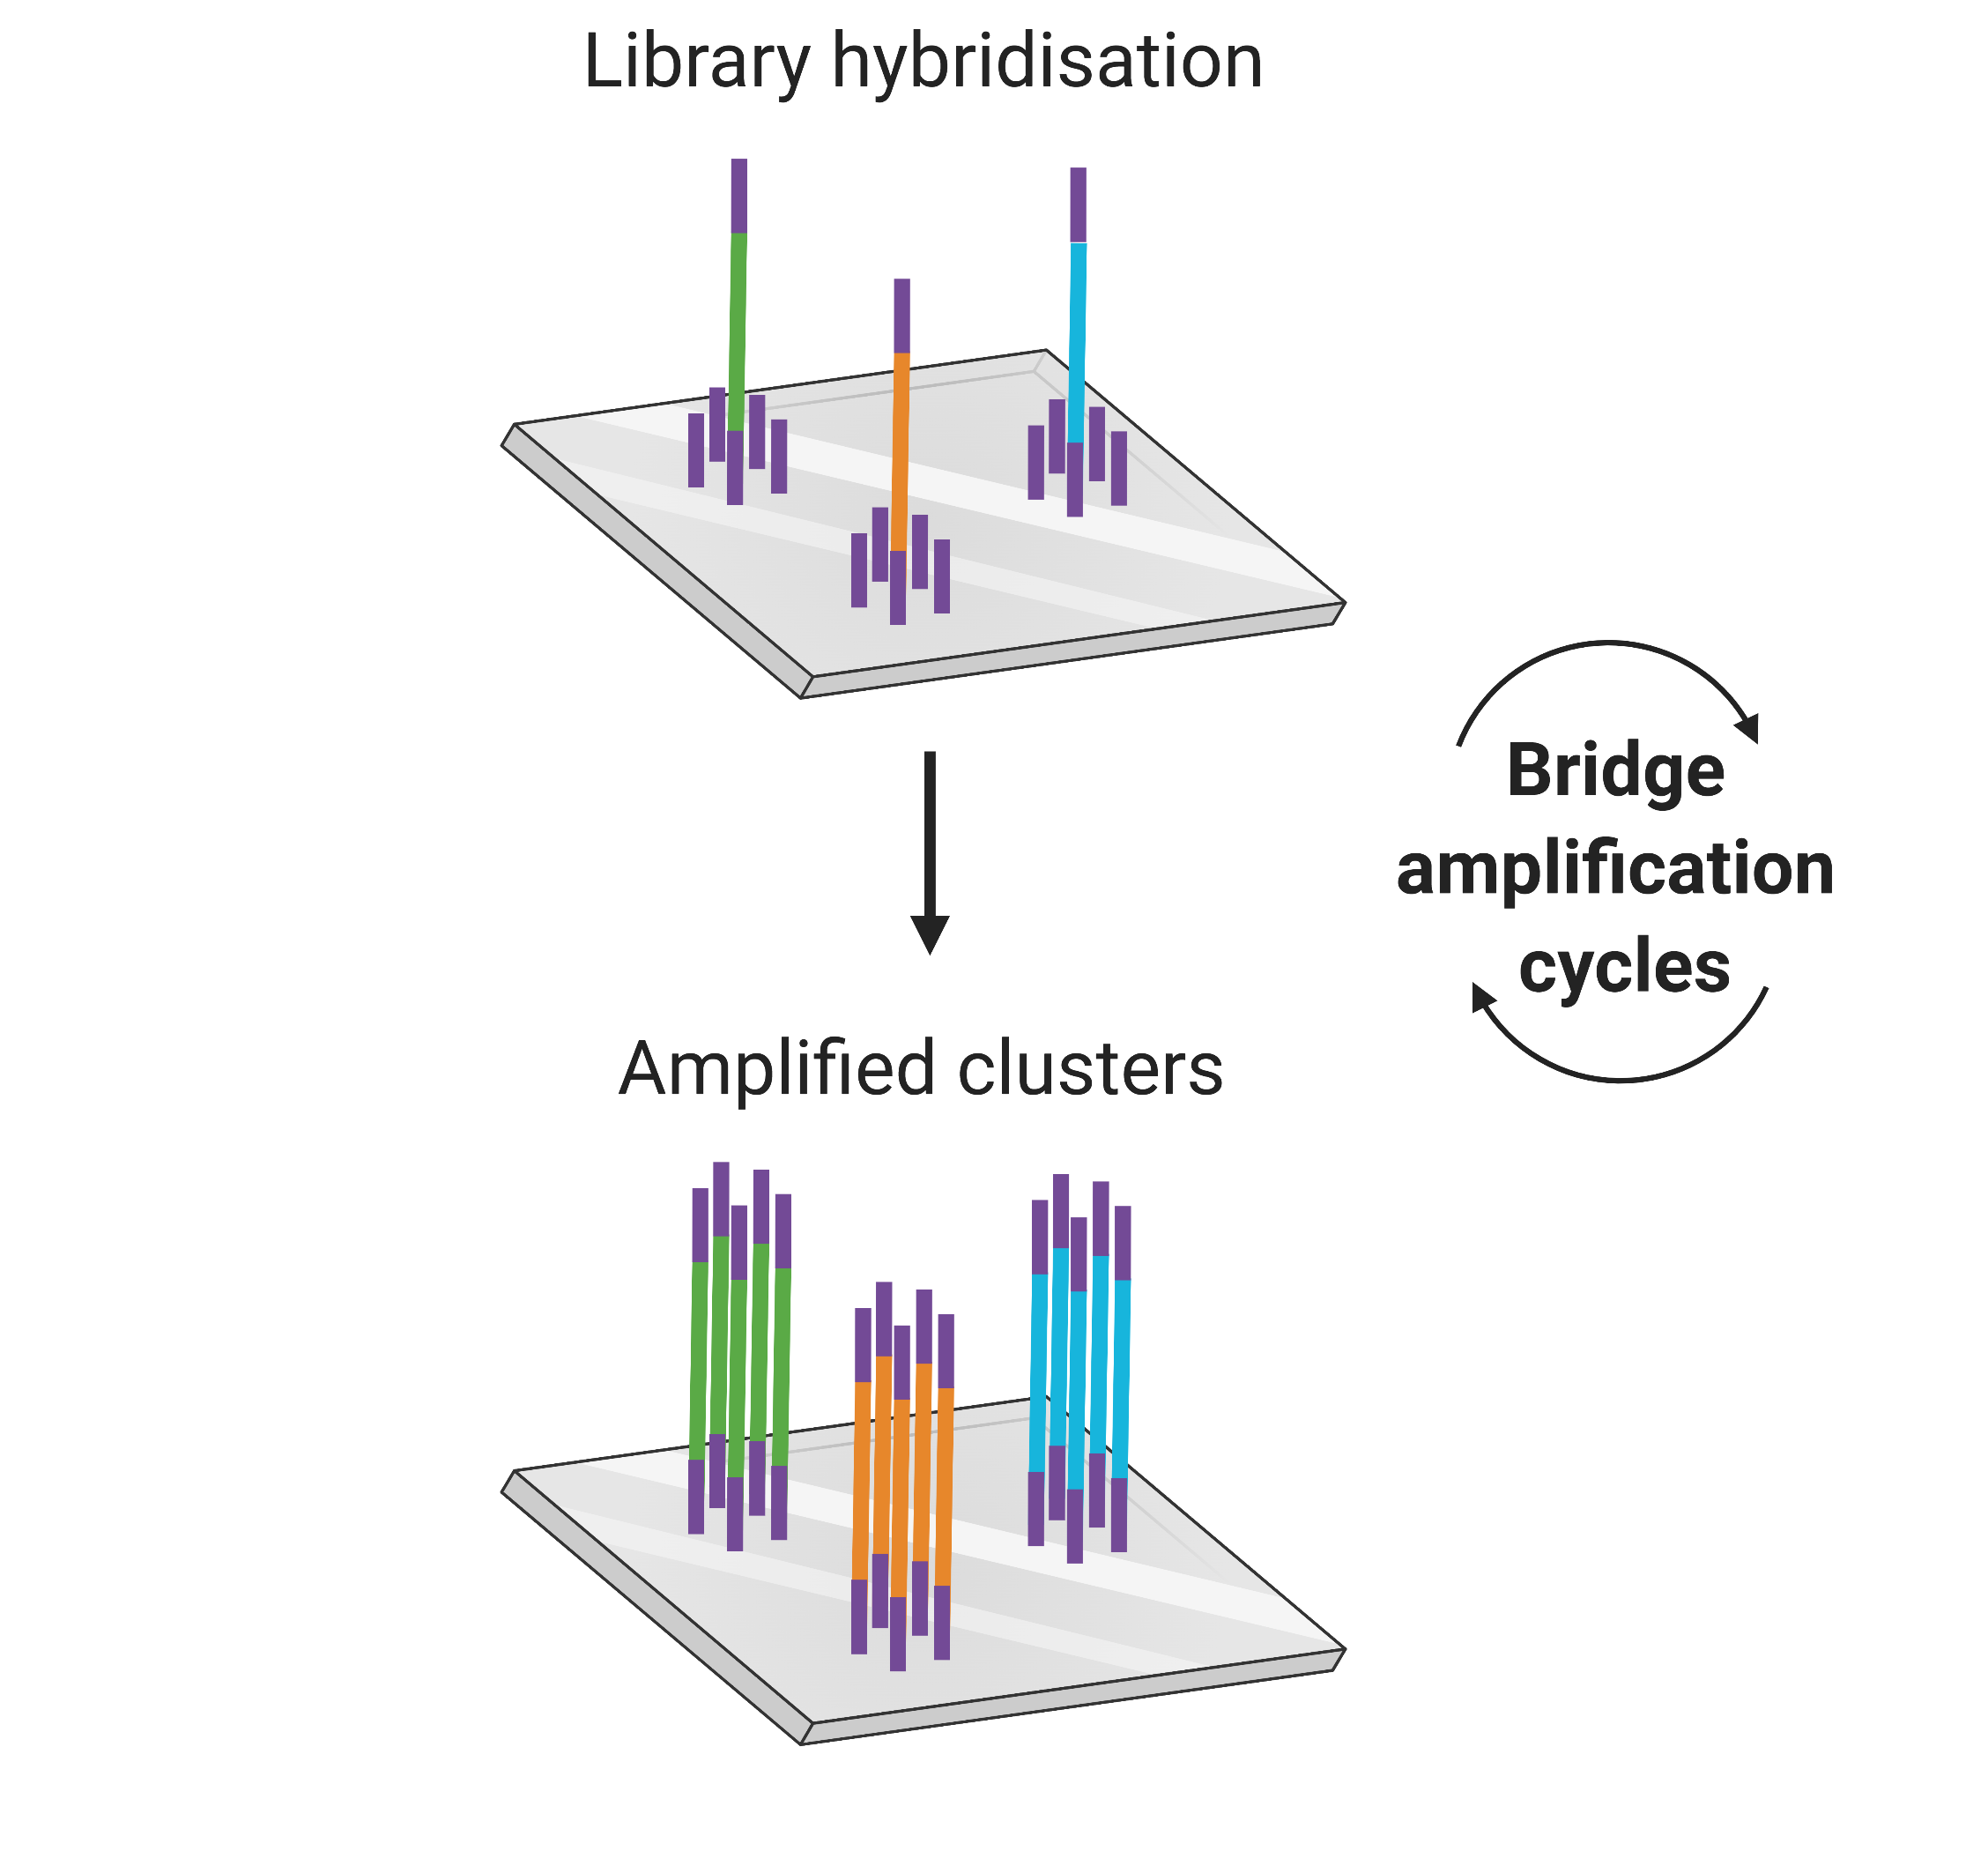
\includegraphics[width=8cm]{ngs_clonal_amp}
    \caption[Illumina clonal amplification]{Illumina clonal amplification. Created using \href{https://biorender.com/}{BioRender.com}. } 
    \label{fig:ngs_clonal_amp}
\end{figure}
\clearpage

\subsection{Sequencing and Nucleobase Detection}
Sequencing by Synthesis \citep{illumina2010} makes use of fluorescently-labelled deoxynucleoside triphosphate (dNTP). Each sequencing cycle binds a dNTP molecule to the millions of clusters in parallel, with each of the four nucleotides emitting a different coloured light upon binding and laser excitation. The sequencing machine captures the light being emitted from the flow cell as an image and identifies the first base of each fragment. The cycle repeats itself for the second base, third base, and so on, until the end of the sequence (\autoref{fig:ngs_sequencing}). The raw sequencing data is stored as Binary Base Call (BCL) files.

Multiple samples may be sequenced simultaneously during a single run, where they are multiplexed by the machine, meaning they are pooled into a single data stream. Unique identifiers called barcode sequences (added to the cDNA fragments during library preparation) allow for the recognition of the different samples, and demultiplexing of the BCL files into text-based FASTQ files \citep{cock2010sanger}. These are immediately compressed to reduce costs associated with data storage and data transfer. While the \textit{de facto} data compression format used is gzip \citep{deutsch1996gzip}, and bzip is used on occasion \citep{seward1996bzip2}, the underlying compression algorithms used are unspecialised and inefficient for genomic data.


\begin{figure}[!ht]
    \centering
    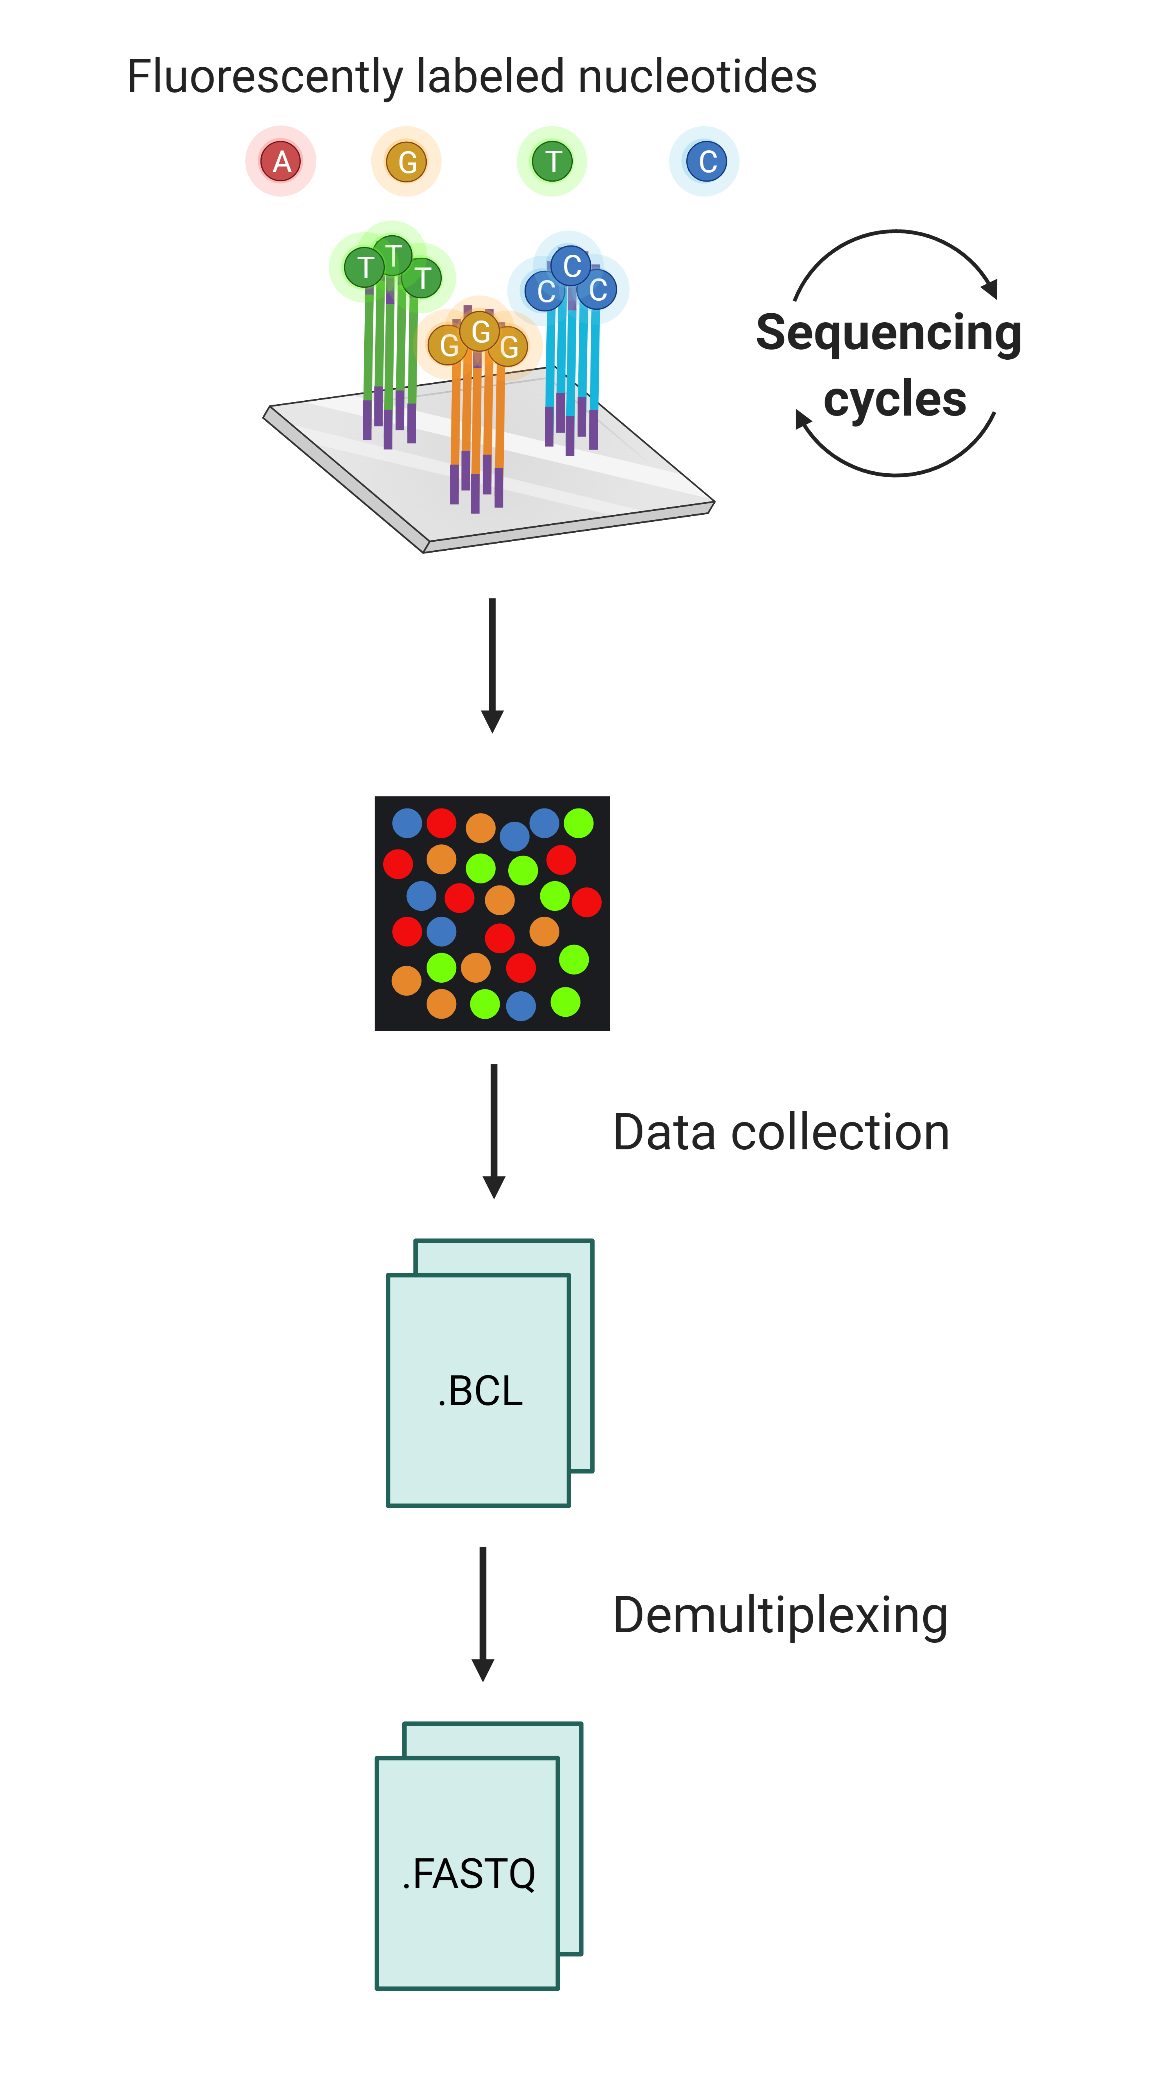
\includegraphics[width=8cm]{ngs_sequencing}
    \caption[Sequencing by synthesis]{Illumina sequencing by synthesis. Created using \href{https://biorender.com/}{BioRender.com}. } 
    \label{fig:ngs_sequencing}
\end{figure}
\clearpage


%illumina sequencing steps: https://www.illumina.com/documents/products/techspotlights/techspotlight_sequencing.pdf
% Potential sequencing errors

%Low complexity regions
%Sequencing software which cannot determine the nucleotide in a particular position, often represent the ambiguous base as 'N'. 
%Potential sequencing errors

% paired end vs single end: Paired-end sequencing sequences both the 5’ and 3’ end of each fragment
% read length
% coverage


\section{RNA-seq: \textit{in silico}}

Once the FASTQ files emerge from the sequencing machines, we may move into the dry lab and feed the data into an RNA-seq data analysis pipeline. While the specific tools which make up the pipeline will vary according to the type of data and goals of the researcher, all RNA-seq pipelines share a common skeleton. The following subsections will first provide a general overview of the respective step in the pipeline, and then delve into the specific tools used in this project.

%Introns are spliced out of the pre-mRNA to form a mature mRNA transcript

\subsection{Quality Control}

The first part of any pipeline should be to analyse the quality of the data received from the sequencing machine. If poor quality sequencing information is identified, it is truncated to mitigate inaccuracies in the downstream pipeline. Some imperfections and uncertainties in sequencing are unavoidable, thus the reading of each base call by the sequencer is assigned a Phred quality score. These are numerical scores generally ranging from 10 to 60, logarithmically related to the probability of an erroneous base-call, represented as a single ASCII character \citep{ewing1998base}. They are calculated as follows:
$$ Q = -10 log_{10}P $$
 $$P = 10^{\frac{-Q}{10}}$$
 
where:
\begin{conditionsenv*}
	Q 		& Phred-scale quality score \\
	P 		& Probability of an erroneous base call \\
\end{conditionsenv*}

A common convention is to write the value of the Phred score after the letter \textit{Q}, so we may say that a base call with quality of Q30 has a 0.1\% chance of being erroneous. The FASTQ files used for this project are Sanger/Illumina 1.9 encoded, meaning that the assigned character to the score is equal to its value as an ASCII code + 33. So Q30 would correspond to the ASCII character with an ASCII code\footnote{The complete Q-score encoding table: \url{https://support.illumina.com/help/BaseSpace_OLH_009008/Content/Source/Informatics/BS/QualityScoreEncoding_swBS.htm}} of 53, which is the question mark character \textit{?} \citep{ewing1998base}. The lack of a base call is represented as an \textit{N} in place of the nucleotide.

\subsubsection{FastQC}
% Useful: https://rtsf.natsci.msu.edu/genomics/tech-notes/fastqc-tutorial-and-faq/#:~:text=FastQC%2C%20written%20by%20Simon%20Andrews,on%20a%20sequence%20data%20set.
In the rapidly changing field of nucleotide sequencing, FastQC \citep{andrews2010fastqc} has been one of the few constants. It has become a staple quality control tool for high throughput sequencing data, accepting BAM \citep{BAM}, SAM or FASTQ files as input, from which it produces an HTML-based report using a number of modules measuring various quality metrics. The software rates each of these modules using a green check-mark signifying that it 'passed' QC, a yellow exclamation mark 'warning', or a red cross 'failed'. However these flags are set to DNA sequencing standards, and have limited applicability with other types of sequencing, such as RNA-seq, where a number are expected to fail. These modules are thoroughly described in its documentation\footnote{\url{https://www.bioinformatics.babraham.ac.uk/projects/fastqc/Help/3\%20Analysis\%20Modules/}} and summarised below. Care should be taken as the X-axis is non-uniform for a number of the produced graphs.

%Maybe add expected moduels to fail
\textbf{Modules used in FastQC:}
\begin{itemize} \itemsep0em
\item \textbf{Basic Statistics} - Some basic information on the file: its name, type of quality score, total read count, read length and GC content.
\item \textbf{Per Base Sequence Quality} - The aggregated Q-scores at each position of the reads, represented by a box-plot.
\item \textbf{Per Sequence Quality Scores} - The number of reads on the y-axis and the average Q-score on the x-axis.
\item \textbf{Per Base Sequence Content} - A relative abundance line graph showing the percentage abundance of each of the four nucleotides across all the reads. 
\item \textbf{Per sequence GC content} - The percentage abundance of each of the four nucleotides across all the reads, overlaid on the expected distribution. 
\item \textbf{Per base \textit{N} content} - Percentage of bases at each position of the sequence with no base call, represented as an \textit{N}.
\item \textbf{Sequence Length Distribution} - Shows the distribution of sequence lengths, measured in number of base-pairs (bp). The module will raise a warning if all sequences are not the same length and an error if any of the sequences have zero length.
\item \textbf{Sequence Duplication Levels} - Percentage of reads in the library which come from sequences with duplication. Two lines indicate the percentages of the raw and the deduplicated libraries.
\item \textbf{Overrepresented Sequences} - A list of sequences which account for $\geq$0.1\% of the total reads. These are compared to common contaminants to try identify them.
\item \textbf{Adapter Content} - A cumulative line graph where a sequence library adapter sequence is identified at that base position.
\end{itemize}

\subsubsection{FastQScreen}
While FastQC is certainly a useful and well-maintained tool, it is not exhaustive of the possible QC metrics for FASTQ files. For this reason, other tools such as FastQScreen\footnote{\url{https://www.bioinformatics.babraham.ac.uk/projects/fastq_screen/_build/html/index.html}} \citep{wingett2018fastq} may be used to supplement the results.

FastQScreen maps the sample reads against the genomes of common contaminants and against that of a human for comparison using a third party alignment tool such as Bowtie \citep{bowtie}, Bowtie2 \citep{bowtie2} or BWA \citep{bwa}. A bar chart (\autoref{fig:fastqscreen_example}) and its respective data table are produced which show the percentage reads mapped for each genome, and what percentage did not map at all. With human samples, one should expect some multi-mapping to the mouse and rat genomes, given their genetic similarities.

\begin{figure}[!ht]
    \centering
    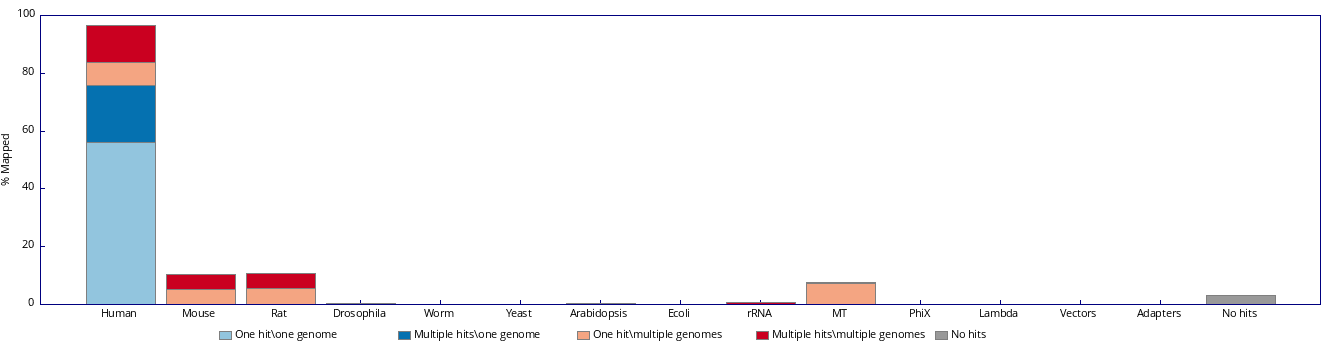
\includegraphics[width=1\textwidth]{fastqscreen_example}
    \caption[FastQScreen plot example]{An example of a good FastQScreen output result, with human mapping close to 100\% and some multi-mapping to mouse and rat genomes. } 
    \label{fig:fastqscreen_example}
\end{figure}
\clearpage

\subsection{Preprocessing}
If poor quality data is identified, it should be cleaned to avoid negative effects in the downstream analysis. Quality trimming which is too aggressive may similarly negatively impact downstream analysis, thus care must be taken to select appropriate quality thresholds \citep{davis2019}.

\subsubsection{Cutadapt: Short reads and Adapter sequences}
\label{cutadapt}
One of the primary functions of Cutadapt \footnote{\url{https://cutadapt.readthedocs.io/en/v4.0/guide.html}} \citep{martin2011cutadapt} (as indicated by its name) is to trim adapter sequences, which may be given as a string following the \texttt{-a} parameter. Additionally, Cutadapt may be given a read length threshold (\texttt{--length}) to remove short reads which are susceptible to multimapping and ambiguity during alignment \citep{deschamps2020handling}. 

Trim Galore!\footnote{\url{https://www.bioinformatics.babraham.ac.uk/projects/trim_galore/}} \citep{trimgalore} is a wrapper script that may be used to instantly redirect the trimmed reads from Cutadapt back to FastQC to reassess the data quality. It accepts the same arguments as Cutadapt, with an additional \texttt{--fastqc\textunderscore args} which accepts additional arguments to be passed on to FastQC as a string. This combines both Cutadapt and FastQC parameters into a single command. 

\textbf{By default Cutadapt:}
\begin{itemize}\itemsep0em
\item Outputs the trimmed FASTQ file and simultaneously generates its FastQC report.
\item Assumes Sanger/Illumina 1.9 quality encoding (ASCII code +33 = Phred score)
\item Trims adapter and up- or downstream sequence
\item Allows a maximum error rate of 10 \% (Error rate = number of errors divided by length of matching region)
\item Removes up to one adapter per read
\item Requires a three nucleotide overlap between read and adapter for an adapter to be found
\end{itemize}


\subsubsection{Prinseq++: Low complexity and No Basecalls}

% PReprocessing and INformation of SEQuence data.
% Useful http://prinseq.sourceforge.net/manual.html
Ambiguity in reads may manifest itself in the form of low complexity regions, and reads with a high number of \textit{N}'s, in addition to those discussed in Section \ref{cutadapt}. The data should be filtered to some degree based on these metrics, which is facilitated by ready-made tools such as Prinseq++ \footnote{\url{https://github.com/Adrian-Cantu/PRINSEQ-plus-plus}} \citep{prinseq++}. Prinseq++ is a C++ multi-threaded implementation of the perl-coded Prinseq-lite software \citep{schmieder2011quality}. 

Regions of low-complexity (also called compositionally biased regions) are a natural part of biological sequences, playing an important role in protein translation \citep{frugier2010low}, and have a functional role in some proteins \citep{ntountoumi2019low}. Nevertheless, due to their repetitive nature, they tend to result in multimapping and low alignment confidence scores, especially when exacerbated with short read lengths. To quantify low-complexity regions, Prinseq++ present the DUST (Tatusov and Lipman, unpublished) and Entropy approaches. Both are different algorithms which employ a scoring function based on nucleotide frequencies which ultimately generate a score between 0 and 1 as a measure for sequence complexity  \citep{morgulis2006fast}. The DUST module is incorporated in BLAST \citep{altschul1997gapped} for the same purpose, to mask low-complexity regions. Prinseq++ filters reads which exceed the stipulated DUST score (\texttt{-lc\textunderscore dust}) or Entropy (\texttt{-lc\textunderscore entropy}) thresholds.

The ambiguous base \textit{N} represents no basecall, and a threshold for the maximum number of \textit{N}'s in a sequence may be set using \texttt{-ns\textunderscore max\textunderscore n}.
    
\textbf{By default Prinseq++:}
\begin{itemize}\itemsep0em
\item Outputs the filtered FASTQ, and the filtered reads as separate files.
\item Removes sequences with a DUST score < 0.5
\item Removes sequences with an Entropy score < 0.5 
\item Trims recursively from both ends of the sequence chunks of length 2 if the mean quality of the first 5 bases is <20 
\end{itemize}

\subsection{Alignment}

There are some semantics associated with this particular step which should be clarified before proceeding. \textit{Alignment} and \textit{mapping} are sometimes used interchangeably, but there are subtle differences. According to the BioStar Handbook \citep{albert2020biostar} and a presentation by Heng Li, \textit{alignment} is the optimal placement of a read against a genome, while \textit{mapping} suggests less certainty, and that the optimal placement is not always possible. Which term to use is dependent on the study, although modern tools often combine the two approaches, which continues to blur the line separating the terms. 

Read aligners are tools designed to perform a pairwise comparison between two sequences, and find regions of high similarity. Aligners may take one of two approached: global alignment or local alignment. Global alignment algorithms, such as \cite{needleman1970general}, aligns both sequences from their first amino acid residue through to their last and is more suitable for sequences of approximately equal lengths. By contrast, local alignment algorithms, such as \cite{smith1981identification} and BLAST, are more suited for sequences that are suspected to overlap only partially.

Alignment algorithm efficiency is at least semi-dependent on read length, with each having ideal range of lengths, although this is rarely stated in the documentation \citep{albert2020biostar}.



% Pseudo aligners vs quasi-aligners
% Reference genomes
% aligning to a genome vs a transcriptome
%Multimapping:https://www.sciencedirect.com/science/article/pii/S2001037020303032

\subsubsection{STAR}
Dobin2013
% reference genome vs transcriptome
% perfect paper: https://currentprotocols.onlinelibrary.wiley.com/doi/abs/10.1002/0471250953.bi1114s51 
% sci hub for it: https://sci-hub.hkvisa.net/10.1002/0471250953.bi1114s51

\cite{dobin2015mapping} provide an excellent overview of potential mapping strategies for using the STAR software package on various RNA-seq data types
It is both a mapping and an alignment tool, since the two terms are used interchangeably in \cite{dobin2015mapping}

\subsection{Read Quantification}


\begin{table}[h]
\centering
\caption{An example of a read count table. Each sample represents the pooled RNA of a large number of cells, often of different cell types.}
\label{tab:read_count}
\begin{tabular}{lllll}
\textbf{Genes} & \textbf{Sample$_{1}$} & \textbf{Sample$_{2}$} & \textbf{Sample$_{3}$} & ...  \\
A2BG  & 10      & 30      & 0       & ...  \\
AML   & 30      & 3       & 3       & ...  \\
AMT2  & 0       & 0       & 10      & ...  \\
ARST5 & 5300    & 1900    & 3250    & ...  \\
...   & ...     & ...     & ...     & ... 
\end{tabular}
\end{table}

\subsubsection{RSEM}
li2011rsem

\subsection{Read Normalisation}
% TPM TMM FPKM RPKM
% https://genomebiology.biomedcentral.com/articles/10.1186/gb-2010-11-3-r25#Sec2

\subsection{Differential Expression Analysis}
% EdgeR and DESeq2
feng2012gfold, gim2016lpeseq, \citep{edger}
%
%Very low read counts cannot be reliably distinguished from background noise so these need to be filtered: https://pubmed.ncbi.nlm.nih.gov/21645359/
\subsubsection{EdgeR}

statistical models used by edger uwekk

\subsection{Downstream Analysis}
% Potential downstream analysis routes
%Functional Annotation
%KEGG kanehisa2000kegg and GO 
%GSEA
%Over-Representation Analysis (ORA)
%Functional Class Scoring (FCS)?
%functional analyses
% alternative splicing, functional analysis, gene fusion detection and eQTL mapping

luo2013pathview

\section{Evaluation Criteria}
%House keeping genes
%Compare DEGs with those found in literature
%future work could perform sanger sequencing

\section{Related Work}
\textbf{In this section you need to explain similar work in literature}.  Make sure to give a systematic overview of studies with related/similar work and highlight similarities/differences to your work (perhaps in the form of a table)

\begin{landscape}
	\pagestyle{empty}
\label{tab:test}
\begin{table}[h]
	\tiny
    \centering
    \captionsetup{font=scriptsize}
    \caption{Studies which compare RNA-seq tools or work-flows, including the tools used at each step and their conclusion summarised to one or two sentences. Those which propose a novel tool were not considered due to their inherit bias.}
    \begin{adjustwidth}{-1cm}{}
    \begin{tabular}{llllllllllllllllll}
		\toprule
        \textbf{Reference} & \textbf{Preprocessing} & \textbf{Mapping} & \textbf{Quantification} & \textbf{Normalisation} & \textbf{Differential expression} & \textbf{Summarised conclusion}  \\ \midrule
        \cite{williams2017empirical} & / &  Bowtie2, HISAT2, Kallisto, & Sailfish, Kallisto,  & / & Ballgown, baySeq, BitSeq,  & Different workflows exhibit a precision/recall   \\ 
        ~ & ~ &  Salmon, Sailfish, SeqMap,  & Salmon & ~ & cuffdiff, DESeq2, EBseq,  & tradeoff,  the method of differential gene  \\ 
        ~ & ~ & STAR, TopHat2 & ~ & ~ & NOISeqBIO, SAMseq, Sleuth,  &  expression exhibited the strongest impact  \\ 
        ~ & ~ & ~ & ~ & ~ & edgeR, limma, NBPseq &  on performance  \\ \hline
        \cite{Zhang2017} & / & Cufflinks, RSEM, TIGAR2,  & Sailfish, Kallisto,  & / & / & Pseudo-aligners require less runtime and   \\ 
        ~ & ~ & eXpress, Sailfish, Kallisto,  & Salmon & ~ & ~ & achieve similar accuracy. Salmon and RSEM  \\
        ~ & ~ & Salmon & ~ & ~ & ~ &  (BAM input) performed the best considering  \\ 
        ~ & ~ & ~ & ~ & ~ & ~ &  computational resources and accuracy  \\ \hline
        \cite{Schaarschmidt2020} & / & BWA, CLC, HISAT2, RSEM,   & RSEM, Kallisto,  &  DEseq & DESeq2, CLC & All mappers can be equally used for RNA-Seq,    \\ 
        ~ & ~ & Kalliso, Salmon, STAR & Salmon,  idxstat, & ~ & ~ & with an outlier being the CLC software combined   \\ 
        ~ & ~ & ~ & featureCounts & ~ & ~ & with it's own differential gene expression module  \\ 
        ~ & ~ & ~ & ~ & ~ & ~ &   \\ \hline
        \cite{MacManes2014} & Trimmomatic,  & Bowtie2  & / & FPKM & / & Suggests a Phred score cutoff of 2 or 5 for    \\ 
        ~ & FastX, BioPieces,  & ~ & ~ & ~ & ~ & transcriptome assembly  \\ 
        ~ & BLAT, Jellyfish & ~ & ~ & ~ & ~ &   \\ 
        ~ & ~ & ~ & ~ & ~ & ~ &   \\ \hline
       \cite{he2020assessing} & Cutadapt, FastP,  & BWA, Novoalign & / & / & / & Differences betwen preprocessing  \\ 
        ~ & Trimmomatic & ~ & ~ & ~ & ~ & techniques are marginal   \\ 
        ~ & ~ & ~ & ~ & ~ & ~ &   \\ 
        ~ & ~ & ~ & ~ & ~ & ~ &   \\ \hline
        \cite{lin2016comparison} & / & / & / & Total Count, & edgeR, DESeq, SAS & Best normalisation approach is to use DESeq and   \\ 
        ~ & ~ & ~ & ~ &  Median, upper  & ~ & model the data using edgeR or DESeq  \\ 
        ~ & ~ & ~ & ~ & quartile, Quantile,  & ~ &   \\ 
        ~ & ~ & ~ & ~ & RPKM, ... & ~ &   \\ \hline
        \cite{everaert2017benchmarking} & / & Tophat, STAR, Kallisto,  & HTSeq, Cufflinks,  & / & / & Each method yielded a small set of lowly  \\ 
        ~ & ~ & Salmon & Kallisto, Salmon & ~ & ~ &  expressed genes  specific to that method  \\ 
        ~ & ~ & ~ & ~ & ~ & ~ &   \\ 
        ~ & ~ & ~ & ~ & ~ & ~ &   \\ \hline
        \cite{srivastava2020alignment} & Trim galore!  & Salmon, STAR, Bowtie2 & tximport, RSEM & DEseq, TMM,  & DESeq2, edgeR, limma & Quasi-mappers are faster but aligners more   \\ 
        ~ & ~ & ~ & ~ & limma & ~ & accurate  \\ 
        ~ & ~ & ~ & ~ & ~ & ~ &   \\ 
        ~ & ~ & ~ & ~ & ~ & ~ &   \\ \hline
        \cite{teng2016benchmark} & / & Flux Capacitor, Cufflinks, & HTSeq, Cufflinks, & / & / & RSEM slightly outperforming the rest with two     \\ 
        ~ & ~ &  eXpress, RSEM, Sailfish, &  Kallisto, Salmon & ~ & ~ & methods clearly under-performing  \\ 
        ~ & ~ &  kallisto, Salmon  & ~ & ~ & ~ &   \\ 
        ~ & ~ & ~ & ~ & ~ & ~ &   \\ \bottomrule
    \end{tabular}
    \end{adjustwidth}
\end{table}
\end{landscape}

Note that this section may be sectioned based on the different aspects of your dissertation.

Talk about papers that used RNA-seq for the treatment of cancers
%file:///C:/Users/matth/OneDrive/Desktop/Msc%20Bioinformatics/!MMB5010%20DISSERTATION-DESKTOP-A2009SI/Literature/Oncology%20of%20AML/LUCIENNE%20Phenolic%20compounds.pdf

%Maybe alter template to include more cells like the template in wikipedia :https://en.wikipedia.org/wiki/Myeloid_tissue#/media/File:Hematopoiesis_(human)_diagram_en.svg






\section{Summary}
